\documentclass[a4paper,12pt]{article}

%% FROM THE PROVIDED math_symbols.tex
\usepackage{amsthm}
\usepackage{amssymb}
\usepackage{amsmath}
\usepackage{mathtools}
\usepackage{xifthen}
\usepackage{xparse}
\usepackage{dsfont}


% Left-right bracket
\newcommand{\lr}[1]{\left (#1\right)}

% Left-right square bracket
\newcommand{\lrs}[1]{\left [#1 \right]}

% Left-right curly bracket
\newcommand{\lrc}[1]{\left \{#1\right\}}

% Left-right absolute value
\newcommand{\lra}[1]{\left |#1\right|}

% Left-right upper value
\newcommand{\lru}[1]{\left \lceil#1\right\rceil}

% Scalar product
\newcommand{\vp}[2]{\left \langle #1 , #2 \right \rangle}

% The real numbers
\newcommand{\R}{\mathbb R}

% The natural numbers
\newcommand{\N}{\mathbb N}

% Expectation symbol with an optional argument
\NewDocumentCommand{\E}{o}{\mathbb E\IfValueT{#1}{\lrs{#1}}}

% Indicator function with an optional argument
\NewDocumentCommand{\1}{o}{\mathds 1{\IfValueT{#1}{\lr{#1}}}}

% Probability function
\let\P\undefined
\NewDocumentCommand{\P}{o}{\mathbb P{\IfValueT{#1}{\lr{#1}}}}

% A hypothesis space
\newcommand{\HH}{\mathcal H}

% A sample space
\newcommand{\XX}{\mathcal{X}}

% A label space
\newcommand{\YY}{\mathcal{Y}}

% A nicer emptyset symbol
\let\emptyset\varnothing

% Sign operator
\DeclareMathOperator{\sign}{sign}
\newcommand{\sgn}[1]{\sign\lr{#1}}

% KL operator
\DeclareMathOperator{\KL}{KL}

% kl operator
\DeclareMathOperator{\kl}{kl}

% The entropy
\let\H\relax
\DeclareMathOperator{\H}{H}

% Majority vote
\DeclareMathOperator{\MV}{MV}

% Variance
\DeclareMathOperator{\V}{Var}
\NewDocumentCommand{\Var}{o}{\V\IfValueT{#1}{\lrs{#1}}}

% VC
\DeclareMathOperator{\VC}{VC}

% VC-dimension
\newcommand{\dVC}{d_{\VC}}

% FAT ...
\DeclareMathOperator{\FAT}{FAT}
\newcommand{\dfat}{d_{\FAT}}
\newcommand{\lfat}{\ell_{\FAT}}
\newcommand{\Lfat}{L_{\FAT}}
\newcommand{\hatLfat}{\hat L_{\FAT}}

% Distance
\DeclareMathOperator{\dist}{dist}

% change all asterisks to \cdots in math mode. use \textasciiasterisk for
% asterisks in math mode.
\DeclareMathSymbol{*}{\mathbin}{symbols}{"01}

% easy integrals over -infinty .. infinity
\newcommand{\infint}{\int\limits_{-\infty}^{\infty}}


%% MY PACKAGES
\usepackage[utf8]{inputenc}
\usepackage[plainpages=false]{hyperref}
\usepackage{cleveref}
\usepackage{graphicx}
\usepackage{minted}    % code snippets
\usemintedstyle{trac}
\setminted{fontsize=\scriptsize, highlightcolor=gray, linenos, frame=lines, framesep=10pt}
% \usepackage{tikz}
% \usetikzlibrary{automata, positioning}
\usepackage[]{xcolor}
\definecolor{gray}{RGB}{235, 230, 222}
\definecolor{myRed}{RGB}{173, 20, 0}
\definecolor{myGreen}{RGB}{45, 150, 0}
\newcommand{\gray}[1]{{\setlength{\fboxsep}{0pt}\colorbox{gray}{#1}}}
\everymath{\displaystyle} % force display style for inline math. why though?


%% My COMMANDS
% big, fat, red TODO's.
\newcommand{\TODO}[1]{\textcolor{red}{TODO: #1}}

\newcommand\numberthis{\addtocounter{equation}{1}\tag{\theequation}} % equation numbering for align*

%% math related commands/operators.

% neat section and subsection separators (but have to insert manually).
\newcommand{\sectend}{\smallskip\noindent\makebox[\textwidth]{\rule{\textwidth}{0.4pt}}}
\newcommand{\Sectend}{\medskip\noindent\makebox[\textwidth]{\rule{1.1\textwidth}{1pt}}}

% easy monospace text for inline code. also,
% no need to escape underscores as with \texttt.
\newcommand{\ms}[1]{\mintinline[fontsize=\normalsize]{text}{#1}}

\DeclareMathOperator*{\argmin}{argmin}

\newcommand{\mbf}[1]{\mathbf{#1}}
\usepackage{geometry}


\newcommand{\concat}{\ensuremath{+\!\!\!\!+\,}}
\newcommand{\rpm}{\raisebox{.2ex}{$\scriptstyle\pm$}}
\newcommand{\resub}[1]{\textcolor{red}{#1}}
\newcommand{\blue}[1]{\textcolor{blue}{#1}}
\newcommand{\ltt}{\sqsubseteq}
\newcommand{\twodots}{\mathinner {\ldotp \ldotp}}

\title{Home Assignment 2\\Machine Learning A}
\author{Anders Holst (wlc376)}

\date{\today}

\newcommand{\ddw}{\frac{\partial}{\partial \, \mbf w}} % partial wrt. w
\newcommand{\tddw}{\tfrac{\partial}{\partial \, \mbf w}} % partial wrt. w, but tiny.

\newcommand{\booltoint}[1]{\llbracket #1 \rrbracket} % bracket notation indicator function.

\newcommand{\mysig}{\theta\!\left[\mbf w^{\text{T}}\mbf x_n\right]} % theta(y_n * w^T * x_n).
\newcommand{\mysigx}{\theta\!\left[\mbf w^{\text{T}}\mbf x\right]} % theta(y * w^T * x).
\newcommand{\meanN}{\frac{1}{N}\sum_{n = 1}^N\,} % 1 / N * sum(n = 1 .. N).

\newcommand{\lnb}[1]{\ln \left\{#1\right\}} % ln {...}

\newcommand{\ywx}{y_n \mbf w^{\text{T}} \mbf x_n} % y_n * w^T * x_n.
\def\stackrel#1#2{\mathrel{\mathop{#2}\limits^{#1}}}
\newcommand{\myeq}{\stackrel{?}{=}}
\newcommand{\myleq}{\stackrel{?}{\leq}}
\newcommand{\mygeq}{\stackrel{?}{\geq}}
\begin{document}

\maketitle

\section{Make Your Own (10 points)}

\begin{enumerate}

  \item \textit{How do you define $\mathcal X$?}

    For each student I would collect current GPA, class attendance, and
    average hand-in page count. Assuming the Danish 7 point grading scale, that
    class attendance is described by a number between 0 and 1, and that page
    count is a natural number, we have $\mathcal X = [-3, 12] \times [0, 1]
    \times \mathbb N$.


  % \item for each prior course taken by the particular student, I would collect
  %   data on the student's lecture/class attendance, assignment point grading
  %
  %   \TODO{what?}. Thus the sample space would be \TODO{$\mathcal X = ...$}.

  \item \textit{How do you define $\mathcal Y$?}

    The label space $\mathcal Y$ would be the set of possible grades --
    assuming the Danish 7 point grading scale, we would have $\mathcal Y = \{-3,
    00, 02, 4, 7, 10, 12\}$.

  \item \textit{How do you define $\ell(y', y)$?}

    I would want incorrect predictions to be punished harder the greater the
    difference between $y'$ and $y$ -- however, to better reduce the number of
    incorrect predictions in the extremes, I would use a square loss function:
    $\ell(y', y) = (y' - y)^2$.

  \item \textit{How do you define $d(x, x')$?}


    Since the three dimensions in $\mathcal X$ have very different ranges, I
    can't use a simple Euclidean distance for $d$, since for one this would weigh
    average page count much higher than class attendance percentage. Instead, in
    order to weigh the differences in all three dimensions equally, I use
    a symmetric relative difference function, and $d$ is defined as:

    $$d(x, x') = \sqrt{\sum_{\substack{i \in \{GPA,\\ attendance,\\ pages\}}}
    \left(\frac{|x_i - x'_i|}{x_i + x'_i}\right)^2}$$

  \item \textit{How would you evaluate your algorithm in terms of $\ell(y', y)$}?

    I am not \textit{entirely} sure that I interpret the question correctly.
    However, I would probably evaluate model accuracy using MSE such that bad
    predictions weigh heavier. Since $\ell$ is a square loss function, the MSE
    is:

    $$
    \frac{1}{n}\sum_{i = 0}^n \ell(y'_i, y_i)
    $$


  \item \textit{Do you expect any issues after deployment?}

    The biggest problem I can imagine is the issue of new students for whom
    there exists no prior data. To alleviate this, I would generate random data
    based on other students (with added random noise, of course).

\end{enumerate}

\sectend
 % DONE
\newpage
\section{Graph-based Image Segmentation}

If we interpret an image as a weighted graph, in which vertices and edges
represent pixels; where vertices are connected if the underlyig pixels are
neighbours in the image; and edge weights represent differences in intensities
between these pixels, then we can employ more sophisticated techniques than the
histogram-based segmentation, and since 3D images are simply graphs with higher
connectivity, the methods generalize nicely.

\subsection{Min-cut Segmentation}

One such graph-based method for segmentation is the \textit{min-cut} method. The
method relies on the property of flot networks\footnote{Note that a flow
network can be represented with a weighted (di-)graph if
the capacity function is embedded into graph edges as weights.}, that the
maximum flow through a network is equal to the total weight of edges in a
minimum cut separating the source and sink terminals\footnote{CLRS\cite{clrs}
has a nice proof of this property (pp. 723-724).}.

This is also called the max-flow/min-cut theorem, and we can exploit it for
segmentation purposes if we define the graph edge weights (ie. the capacity
function) in such a way that similar pixels share a \textit{high} capacity edge,
and edges between contrasting pixels have \textit{low} capacity.

As with threshold segmentation some user input is at this point required, in the
form of seed pixel coordinate(s) denoting source(s) and sink(s) for a particular
object. By choosing seeds inside and outside of a desired segment, respectively,
the algorithm will analyze the flows running from the object and out and produce
a min-cut along the edge of the object -- flooding can then be
used to label pixels inside the border denoted by the min-cut. 

\medskip

Ideally, that is -- if seeds are well-chosen, this will be the case. As Grady
notes in \cite{grady}, a successful segmentation is practically guaranteed given
enough user inpupt -- however, a number of different problems can arise from
incorrect seeding. The most promiment of these is the ``small cut problem'', a
consequence of under-seeding, in which the algorithm will simply select a cut
involving a very small number of edges close to a seed vertex, since cutting a
small number of high-intensity edges can in many cases be cheaper than cutting a
large number of low-intensity edges. This is rectifiable but requires
additional, or better placed, seeding \cite{grady}.


% \TODO{choose 0 or 1 of these out-commented paragraphs!}
% Another disadvantage of the method is the fact that only a single, contiguous
% object can be segmented at a time, meaning disjoint objects which we would
% identify as coherent (eg. a pair of lungs or parallel arteries) would
% have to be segmented separately.

% Another disadvantage is that since there can exist many cuts with capacities near
% the min-cut, and even multiple min-cuts, the amount and placement of seeds, as
% well as small changes in the image (eg. noise) can result in entirely different
% results from the algorithm.

\subsection{Random Walker Segmentation}

As a remedy to the disadvantages of min-cut segmentation, Leo Grady formulated
Random Walker Segmentation (henceforth, RW) as an alternative graph-based
algorithm in \cite{grady}. Rather than using seeds to partition the graph, RW
computes the probability than any given pixel be associated to any given seed,
for each seed in the image, and labels each pixel according to the seed with
which it is most likely to be associated.

These probabilities are based on the same edge capacities as before, and do not
involve (pseudo-)randomness, but it is beneficial to model the problem using
probabilities. However in some simplified terms the highest probability
terminating seed for a given random walker can be thought of as the seed
for which the mean edge capacities on the path from pixel to seed are maximized.


\medskip

Below figure \cref{fig:RW-seg} shows RW segmentation of the same example image
as before, for two different levels of seeding and two different
parameterizations of the RW motion probability function.


\begin{figure}%[H]
  \includegraphics[width=0.8\textwidth]{figures/RW_segmentation.png}
  % \vspace{-0.8cm}
  \caption{\small \textit{Comparison of RW for different amounts of
  seeding and different beta (penalization coefficient for the RW motion
  function). The sparse seeding is a random sample
  of the full seed pool. Note how segment 4 (yellow) is split in two disjoint
  objects.}}
  \label{fig:RW-seg}
\end{figure}

Obviously noise in the input image makes the segmentation less precise, but one
advantage of RW (and graph-cut, too) is that with good seeding, the output
segmentation is already de-noised as opposed to histogram segmentation.

As the plot shows RW is also very sensitive to proper seeding: The disjoint
segment 4 (yellow) is not properly segmented when its annex is not seeded
(bottom row). Even if the solution is simply more seeding, this is still a
disadvantage. Perhaps the biggest disadvantage of RW, however, is a huge
sensitivity to proper parameterization of the RW motion probability function
(ie. the probabilities attached to each edge in the graph), as is also evident
in the plot, where the segmentation is, to put it mildly, hit and miss depending
on beta (see caption).



\sectend

\iffalse{
Section 2 (L2C, L2D) -- graph cut and random walker algorithms for segmentation -- 
* graph cut: finding minimum cut via max flow.
  the max-flow/min-cut theorem states that the maximum flow through a graph
  is equal to the minimum sum cut.

  in graph cut segmentation, we denote capacity of an edge between two pixels as
  the difference in pixel intensities; as an example, the edge between two
  (neighbouring) black pixels would have higher capacity than would the edge
  between a black and a white pixel.

  By choosing a source pixel (or \textit{seed}) inside of a given object, aswell
  as a target seed \textit{outside} of that object (ie. in the background of the
  image), the border of the object will, if the seeds are chosen correctly and
  the algorithm is successful, be the min-cut of the image graph.

  the problem: works only if we have one object and a background.

* random walker

  can segment multiple objects and several backgrounds.
  ??

  % we call it a \textit{random} walker, but a good way to think about the
  % algorithm is to call it a \textit{minimizing} walker, and, in fact, there is
  % not one but \textit{many} such ``walkers''

  show example of random walker segmentation

* both random walker and graph cut assume that objects in the image form in
  contiguous clusters -- this implies that to segment multiple related objects,
  each need to be properly and individually seeded, whereas with histogram based
  segmentation we can simply choose a good threshold and capture all desired
  objects -- on the other hand, if used properly then graph based segmentation
  can more easily filter out unwanted noise without the need for CCD.

}\fi
 % mangler.
\newpage
\section{\underline{A4.3}}

\subsection{A4.3.a}

\begin{itemize}
  \item \emph{Describe how the syntax of each expression in the Troll grammar is
    represented as embedded syntax in PLD LISP. Discuss nontrivial choices.}
\end{itemize}


\subsubsection{The embedded syntax}

In this subsubsection, I discuss how the Troll syntax is embedded into the
PLD-LISP language. Please note that I do not explain the embedding of each and
every single constructor, but rather only discuss \emph{non-trivial} choices
made - \textbf{where nothing else is stated, the embedded syntax can thus be assumed to
resemble actual Troll syntax.}


\paragraph{On parsing in PLD-LISP}~\smallskip

With limited pattern matching in PLD-LISP (we can only match the first $n$
elements and the tail of a list, not a recursive pattern eg. with ML-like
datatypes), my first thought was that it might at least be possible to implement
an LL1-parser for Troll. However, the parsing table very quickly became very
large and contrived on paper and so I gave up.

\smallskip

I instead pursue implementing a simple evaluator for fully parenthesized Troll
expressions (with the exception that parentheses can be omitted around
single-symbol expressions).


\paragraph{Embedding the Troll syntax}~\smallskip

A Troll expression is represented as a single, nested list of PLD-LISP symbols
and number constants. Troll operators and keywords (\ms d, \ms{accumulate},
\ms{+}, \ms{count}, etc.) as well as variables are simply represented with
symbols. Aside from one restriction and one deviation to the Troll syntax (which
will be discussed momentarily), \emph{the only distinguishing factor is this
enclosing PLD-LISP list.}


\paragraph{Restrictions to the embedded syntax wrt. whitespace and
parenthesization}~\smallskip

As mentioned above, expressions must be parenthesized if they contain more
than one symbol - this for example means that the singleton collection
containing the number 43 can be represented as both the singleton list
\ms{'(43)} and simply the constant ``\ms{43}'' (and similarly for variables),
whereas a Troll expression such as \ms{d x d3} must be parenthesized as
\ms{'(d(x d 3))}\footnote{Also, please note the explicit whitespace between the
inner \texttt d and its second parameter \texttt 3, which is required since
otherwise the two would be recognized as the single symbol ``\texttt{d3}'', much
like how Troll itself requires whitespace between \texttt d and \texttt x.}.
This is because evaluation of dice rolling is \emph{largely} implemented as
such:

\begin{minted}[linenos=false]{lisp}
(define eval
  (lambda (('d e))     (roll 1 (eval e))
          ((e1 'd e2)) (roll (eval e1) (eval e2))
          ...
\end{minted}

\emph{(Note that this snippet is pseudocode and not actual implementation
\footnote{The actual evaluator is also parameterized with the current
environment, and will for example assert that \texttt{eval e} is a singleton
collection containing one positive number.}. More on this later.)}

\smallskip

Here, the \ms{('d e)} pattern matches \emph{precisely} one literal ``\ms d''
followed by exactly one single value (a symbol or list or symbols), so we must
parenthesize \ms{2 d x} since this consists of three distinct symbols. We
\emph{could} rewrite the \ms{d e} pattern to use a head/tail pattern as such:

\begin{minted}[linenos=false]{lisp}
(define eval
  (lambda (('d . es))    (roll 1 (eval es))
          ((e1 'd . es)) (roll (eval e1) (eval es))
          ...
\end{minted}

Using these patterns enables us to evaluate lists such as \ms{'(4 d d d 3 + 4)}
- but this only works because the dice rolling operators are right-associative,
and because the head of the head/tail pattern is matched \emph{exactly};
unfortunately, this approach falls short for lists such as \ms{'(3 + 4 d d 5)},
since the pattern \ms{e1} cannot match the three symbols constituting \ms{3 +
4}.

\smallskip

Different problems arise with other operators with multiple parameters, in
particular the \ms{accumulate} expression, which interleaves multiple keywords
and expressions. Thus, to ease implementation, I give the restriction that any
Troll operator which takes $n$ parameters will in the embedded syntax take
exactly $n$ symbols or lists of symbols.

\newpage

All in all this makes for a great deal of redundant parenthesization in the
embedded syntax. For a more contrived example, consider the Troll expression:

$$\ms{sum least 20 accumulate x := d42 d d d1337 while 888 < sum largest 19 x}$$

In the embedded syntax, this is represented by the nested PLD-LISP list:

\begin{align*}
  \ms{'(sum (least 20 (}&\ms{accumulate x := ((d 42) d (d (d 1337)))}\\
  &\ms{while (800 < (sum (largest 19 x))))))}
\end{align*}

On the other hand one might argue that in some cases parenthesization benefits
code legibility - because even if association and precedence is well-defiend for
all Troll operators, it can sometimes be hard for a human programmer to decipher
from a glance of the code, eg. as with the example given here.

\subsubsection{Deviation in the embedded syntax wrt. union expressions}

Aside from full parenthesization and some forced whitespace, my embedded syntax
deviates from that of the given syntax in one other place: The union syntax,
$\{\ms e_1,\; \dots,\; \ms e_n\}$, which, in Troll, is given by zero or more
comma separated Troll expressions enclosed in curly braces. In the embedded
syntax, a union is simply a PLD-LISP list containing zero or more comma
separated expressions. As an example, the Troll expression \ms{{3 + 4, 4 d 19,
choose {42, 43}}} is represented in the embedded syntax as:

$$
\ms{'((3 + 4), (4 d 19), (choose (42 , 43)))}
$$

Notice the explicit whitespace surrounding the last comma; as per usual,
whitespace is not required around commas in the presence of parentheses, but
\emph{is} required in all other cases since commas are merely PLD-LISP symbols,
and other symbols are free to ``absorb'' those commas if there is no separating
whitespace.

\bigskip

Question: \emph{Why not use curly braces as in the source syntax?}

Answer: In order to use curly braces to denote unions in the embedded syntax,
these would have to be represented as separate PLD-LISP symbols. This, I felt,
overly complicated the embedded syntax, especially considering that to properly
evaluate a union expression in the absence of a parser, the curly braces would
have to be treated as any other symbol in terms of whitespace and
parenthesization. For example, the Troll expression \ms{least 2 {1, 2, {3, 4}}}
would necessarily be represented by the nested list:

$$
\ms{'(least 2 ({ 1 , 2 , ({ 3 , 4 }) }))}
$$

with whitespace even between the opening brace and first expression, as well as
between the last expression and closing brace (again, unless these are
parenthesized), whereas by using PLD-LISP lists to implement the syntax, this
expression is simply:

$$
\ms{'(least 2 (1 , 2 , (3 , 4)))}
$$

To evaluate an empty union, simply give an empty PLD-LISP list ;)


\sectend

\newpage
\subsection{A4.3.b}

\begin{itemize}
  \item \emph{Implement the subset of Troll as presented in the assignment text.
    Discuss non-trivial choices.}
\end{itemize}

\subsubsection{Implementation overview}

I have (to the best of my knowledge) successfully implemented evaluation of
every expression in the Troll subset as embedded syntax in the PLD-LISP
interpreter. As explaiend ealier, I have not implemented any sort of parser, so
the former only holds under the assumption of full parenthesization.

\smallskip

Aside from handling each constructor given in the grammar, my implementation
handles:

\begin{itemize}
  \item specifying a number of isolated rolls, which are then returned as a
    collection of collections;
  \item correct variable binding, including dynamic scoping and variable
    overshadowing;
  \item flattening of arbitrarily nested collections of collections (with the
    exception of specifying multiple rolls, where a single collection of flat
    collections is returned).
\end{itemize}

I claim neither efficiency nor exhaustive correctness (I will, however, make an
effort of testing later), but my implementation \emph{does} handle the following
cases of run-time errors:

\begin{itemize}
  \item non-singleton collection used where singleton collection expected
  \item (singleton collection containing a) non-positive value used where (singleton
    collection containing a) positive value expected
  \item unknown variable names
\end{itemize}

The implementation consists of one large evaluator function, \ms{eval}, and a
number of helper functions. In the following subsubsection, I go into detail
with most of the features mentioned above, as well as other interesting features
of the code.

\smallskip

The code can be viewed in its entirety in the attached \ms{Troll.le} of the code
hand-in directory.

\subsubsection{Non-trivial implementation details}

\paragraph{Randomness}~\smallskip

My handling of randomness is entirely trivial, but I see it fit to mention that
for the sampling and accumulation operators (which both evaluate some of their
operand expressions multiple times, with different, random results each time),
randomness is achieved by passing expressions \emph{unevaluated}, such that they
can be re-evaluated with new random results.

\paragraph{Variable environment}~\smallskip

To implement dynamic scoping, I let my main evaluator function take an
additional parameter \ms{env} holding the local variable environment.
Unfortunately, this parameter must be passed explicitly, which has lead to
cluttered code and, during implementation, a great deal of errors.

\smallskip

Troll variable binding and lookup expressions are handled as such:


\begin{minted}[highlightlines={6, 10}]{lisp}
(define eval
  (lambda ...

    ; variable binding. v must be a symbol; e1 and e2 are arbitrary exps.
    ((v ':= e1 '; e2) env) (if (symbol? v)
                               (eval e2 (bind v (eval e1 env) env)))
    ...
    ; scalar expression. symbols are assumed to be variables, while
    ; singleton collections are created from scalar numeric values.
    (x env)  (if (symbol? x) (lookup x env) (if (number? x) (list x)))
  )
)
\end{minted}

In line 6, the current \ms{env} is extended with a binding of \ms{v} to
whichever value \ms{e1} evaluates to, before \ms{e2} is evaluated under this new
environment. Line 10 shows how symbols are looked up as variables. Note that
this is the bottom-most production of the \ms{eval} function.

\medskip

The actual variable environment \ms{env} is implemented as a list of two-element
PLD-LISP lists whose first element is a symbol and whose second element is a
fully evaluated collection. I omit the code for binding and lookup as it is
entirely trivial, except to say that variable overshadowing is implemented by
always prepending variables to the head of the environment list.

\paragraph{Singleton collections}~\smallskip

A number of Troll operators expect one or more singleton collections as
operands; for example, the arithmetic operators and the multiple dice roll
expects that \emph{both} operands are singleton, while the sample operator
expects its first operand to be.
Furthermore, we also have operators which expect singleton collections
containing positive values - examples of this are dice rolls and
\ms{least/largest}.

\smallskip

This is implemented using two wrappers for the main \ms{eval} function, called
\ms{evalST} and \ms{evalSTPos} (for ``evaluate singleton [positive]''), which
both evaluate its first argument expression and return empty lists (to signal
failure) when the result is not a singleton collection or a singleton collection
containing one positive value, respectively.

\paragraph{Flattening collections}~\smallskip

The Troll manual specifies that nested collections of collections are always
flattened. This is relevant for the sampling, union, and accumulate
expressions, which produce multiple, isolated collections before flattening into
a single collection.

Since collections are implemented as PLD-LISP lists, I write a generic function
for the flattening of arbitrarily nested and arbitrarily irregular PLD-LISP
lists (the function is called \ms{flatten} in the code hand-in), which can then
be used to wrap the result of a sampling, accumulation, or union expression.

\paragraph{Union expressions}~\smallskip

An example of collection flattening is in the union expression $\{\ms e_1,
\dots, \ms e_n\}$. 

As explianed earlier, I use simply PLD-LISP lists to represent Troll unions. To
evaluate arbitrarily long union expressions, I give \ms{eval} a head/tail
pattern as seen below:

\begin{minted}[highlightlines={6}]{lisp}
(define eval
  (lambda
    ...
    ; {e1, ..., en}: this production assumes n > 0; to create an empty collection,
    ; simply give an empty list. for example, '(count ()) evaluates to (0).
    ((e ', . es) env)  (flatten (cons (eval e env) (eval es env)))
    ...
\end{minted}

Notice how the same \ms{env} is used for each expression, and how the resulting
union is created using \ms{flatten}. The code comment explains the case of empty
unions.


% \paragraph{Collection (ie. list) operators}~\smallskip
%
% The implementation of \ms{sum}, \ms{min}, \ms{max}, \ms{count}, and the
% filtering
%
% To implement the collection operators \ms{sum}, \ms{min}, \ms{max}, and
% \ms{count}, I first implement generic list \ms{map} and \ms{reduce} functions.
% The first three operators are then implemented as reductions using addition, and
% binary min and max and their respective neutral elements. \ms{count} is
% simply implemented using the built-in \ms{length}.
%
% \medskip
%
% Similarly, list filtering is implemented using a generic \ms{filter} function,
% the code of which I shall also omit as it is trivial.


\paragraph{\texttt{least} and \texttt{largest} expressions}~\smallskip

\ms{least} and \ms{largest} are both implemented using a simple (ie. not
in-place) quicksort. To pick the \ms n least elements of some collection
\ms{xs}, the collection is first fully evaluated and sorted before the first
$\ms{min(n, count xs)}$ elements are extracted; for the \ms n largest, the list
is reversed after sorting.


\paragraph{\texttt{accumulate} expression}~\smallskip

Below snippet shows how \ms{accumulate} expressions are evaluated (interesting
lines highlighted):

\begin{minted}[highlightlines={4, 5, 12-14}]{lisp}
(define eval
  (lambda
    ...
    (('accumulate v ':= e1 'while e2) env) 
      (if (symbol? v) (flatten (accumulate v e1 e2 env)))
    ...
  ...
...

(define accumulate
  (lambda
    (v e1 e2 env) (if (define x (eval e1 env))
                      (cons x (if (eval e2 (bind v x env))
                              (accumulate v e1 e2 env))))
  )
)
\end{minted}

Lines 4-5 show how \ms{accumulate} expressions are matched in the main evaluator
function; if \ms{v} is a symbol, expressions \ms{e1} and \ms{e2} are passed
\emph{unevaluated} to a helper function for accumulation expressions.

\medskip

Given a symbol \ms{v}, two \emph{unevaluated} expressions, and the current
environment \ms{env}, the \ms{accumulate} helper function works as such:

\begin{itemize}
  \item evaluate \ms{e1} under \ms{env} and bind result to \ms{x} (PLD-LISP
    variable);
  \item evaluate \ms{e2} under the environment \ms{env[v -> x]};
  \item accumulate \ms x, and, if \ms{e2} evaluates to a non-empty collection;
    recurse with \ms{e1} and \ms{e2} again unevaluated, and using the original
    \ms{env} (ie. without the binding of \ms{v -> x}).
\end{itemize}

Note the \ms{if}-expression beginning on line 12 of the snippet. This is to
sequence the binding of \ms{eval e1 env} to the PLD-LISP variable \ms{x} before
recursing, such that \ms{e1} is only evaluated once. This works because
\ms{define} is always successful (which it is because \ms x is not a reserved
name in PLD-LISP).

\sectend


\newpage
\subsection{A4.3.c}

\begin{itemize}
  \item \emph{Write a short guide to usage of your implementation. Show example
    rolls by generating at least 10 rolls of each example Troll expression given
    in the assignment text.}
\end{itemize}

\subsubsection{User guide}

To boot up my embedded Troll interpreter implementation, use \ms{make run} from
within my code hand-in directory; alternatively, load the module manually by
evaluating \ms{(load Troll)} from the PLD-LISP interpreter.

\medskip

The API of my evaluator is simply the function \ms{troll}.
To evaluate some Troll expression \ms e (where \ms e is given in the embedded
syntax), use \ms{(troll e)}. To roll \ms e multiple times - say, \ms n times,
each with different random results; use instead \ms{(troll n e)}.

\subsubsection{Example rolls}

In below snippet, I evaluate the example rolls given in assignment text,
followed by 7 rolls of the the example Troll expression discussed earlier:

\begin{minted}[linenos=false]{lisp}
> ; 10 rolls of `d12+d8`
  (troll 10 '((d 12) + (d 8)))
> = ((10) (13) (13) (8) (14) (12) (2) (9) (17) (7))

> ; 10 rolls of `min 2d20`
  (troll '(min (2 d 20)))
> = ((5) (3) (7) (13) (9) (12) (3) (4) (13) (8))

> ; 10 rolls of `max 2d20`
  (troll 10 (max (2 d 20)))
> = ((11) (20) (17) (8) (10) (20) (17) (20) (19) (18))

> ; 10 rolls of `sum largest 3 4d6`
  (troll 10 '(sum (largest 3 (4 d 6))))
> = ((12) (14) (14) (9) (4) (15) (11) (10) (13) (8))

> ; 10 rolls of `count 7 < 10d10`
  (troll 10 '(count (7 < (10 d 10))))
> = ((3) (5) (3) (3) (1) (3) (3) (3) (1) (4))

> ; 10 rolls of: `choose {1, 3, 5}`
  (troll 10 '(choose (1 , 3 , 5)))
> = ((5) (5) (3) (5) (3) (5) (3) (1) (3) (1))

> ; 10 rolls of `accumulate x := d6 while x > 2`
  (troll 10 '(accumulate x := (d 6) while (x > 2)))
> = ((3 4 4 1) (2) (6 4 5 3 2) (4 1) (6 4 4 1)
      (5 6 5 5 4 4 5 3 6 6 3 3 3 6 3 1) (3 6 4 1) (4 2)
      (3 5 2) (4 3 3 4 6 4 5 6 2))

> ; 10 rolls of `x := 3d6 ; min x + max x`
  (troll 10 '(x := (3 d 6) ; ((min x) + (max x))))
> = ((3) (11) (9) (3) (6) (9) (8) (6) (7) (5))

> ; 7 rolls of the example discussed in the report wrt. parenthesization
  (troll 7 '(sum (least (19 + 1) (accumulate x := ((d 42) d (d (d 1337)))
  while (800 < (sum (largest 19 x)))))))
= ((782) (1250) (175) (1212) (418) (170) (277))
\end{minted}

To reproduce these example rolls, use \ms{make example} from within the code
hand-in. The output will not include the same annotations as above snippet.


\newpage
\subsubsection{Testing}

In addition to the example rolls, I want to test my program. Ideally, I would
write automated and reproducible unit tests, but this is only feasible for Troll
expressions with no randomness involved; for dice rolling (ie. \ms d $e$ and
$e_1$ \ms d $e_2$) and the \ms{choose} operator, manual testing will have to
suffice \footnote{In a different setting or scope we might have used eg.
quickcheck testing.}. I also perform manual testing of the \ms{accumulate}
expression, since if there is no randomness involved then we can only have one
accumulation \emph{or} infinite looping.

\paragraph{Manual testing of random operators}~\smallskip

Below are the test cases used in my manual testing of random operators. I hope
that the prompt print-out speaks for itself.

\begin{minted}{lisp}
> (troll '(d 400))    ; single die roll.
= (276)               
> (troll '(d 1))      ; single one-sided die roll.
= (1)                 
> (troll '(d -12))    ; invalid single die roll.
= ()

> (troll '(23 d 400)) ; multi dice roll.
= (197 341 318 240 79 387 121 318 121 113 287 86 131 211 12 216 116 53 166 120 
   202 11 112)
> (troll '(1 d 19))   ; multi dice roll, but just one die.
= (8)
> (troll '(0 d 19))   ; no dice!
= ()

> (troll '(choose (1 , 2 , 3 , 4 , 5))) ; simple choose expression.
= (2)
> (troll '(choose (1843 d 5000000)))    ; choose among many.
= (4533089)                             
> (troll '(choose (d 1)))               ; choose from singleton collection.
= (1)                                   
> (troll '(choose (50 < (4 d 19))))     ; choose from empty collection.
= ()

> (troll '(accumulate x := (65 < (10 d 100))  ; simple accumulate expression
                      while (1 < (count x)))) ; which runs for multiple iterations.
= (91 76 81 98 82 66 100 75 94 78 99 96 75 91 100 77 87 90 83 80 97 79 87 87 86
   66 77 97 95 83 76 80 82 96 74 88 93 83 97 100 90 81 66 76 99 98 95 66 73 82
   97 97 74 90 93 76 88)
\end{minted}

The results seem reasonable - all values are within expected ranges, and the
sizes of all produced collections are as expected. To reproduce, use \ms{make
manual_tests} from within the code hand-in.

\paragraph{Unit testing}~\smallskip

I write small and simple unit tests for the rest of the constructors in the
subset of Troll. I attempt to also test various features of the Troll language,
such as correct flattening of collections in collections, correct variable
scope, and variable overshadowing, as well as a small number of edge case use
cases, such as empty collections, illegal dice rolls, and unknown variables.

\smallskip

I do \emph{not} write any tests of syntactically invalid programs.

\medskip

All my test cases run successfully. Test cases can be viewed in the
\ms{testing.le} file of my code hand-in, and test results can be reproduced with
\ms{make unit_tests} from inside the code hand-in directory.

\medskip

To reproduce all tests, use instead \ms{make test}.

\sectend

\subsection{A4.3.d}

\begin{itemize}
    \item \emph{If there is anything missing, discuss how this might be
      resolved.}
\end{itemize}

I am fairly certain that my implementation correctly handles all expressions in
the subset of Troll given in the assignment text. However, I for one cannot
guarantee that my implementation is bugfree.

\smallskip

More importantly, my implementation only works under the assumption of full
parenthesization of the embedded syntax. This is quite a huge assumption! To
remedy this, I would look into implementing an actual parser for the language.
In this regard, I again argue that PLD-LISP's head/tail pattern matching lends
itself best to a LL1-parser with stack-based AST generation. Given more time, I
would have liked to have given a better attempt at this - in hindsight, I would
have done better to have used an automatic parser table generator rather than
attempting (and quickly failing) at doing this by hand.

\Sectend

 % DONE -- skal skrives ind.
\section{Random Forests}

\subsection{Analyzing satellite data}

\subsubsection{Building, training, and evaluating the model}

In the attached \texttt{code.py}, I build and train a random forest model on the
training data using \texttt{sklearn.ensemble.RandomForestClassifier}. Below
snippet shows the most important bits:

\begin{minted}{python}
train_data = np.load(data_dir + "landsat_train" + data_extension)
train_y = train_data[:, 0]
train_X = train_data[:, 1:]
RFC = RFClassifier(n_estimators = 10,  # 10 trees in forest.
                   criterion = "gini", # use Gini impurities.
                   bootstrap = True,   # use bootstrap samples.
                   max_depth = None,   # build full trees.
                   n_jobs = -1,        # might aswell parallelize.
                   random_state = 2,   # for reproducibility.
                  )
RFC.fit(train_X, train_y)
\end{minted}

Next, I use the trained model to predict the labels for the validation set as
such:

\begin{minted}{python}
validation_data = np.load(data_dir + "landsat_validation" + data_extension)
validation_y    = validation_data[:, 0]
validation_X    = validation_data[:, 1:]

predictions = RFC.predict(validation_X)
accuracy    = np.mean(predictions == validation_y)
\end{minted}

And I find the validation accuracy to be 0.751.

\subsubsection{Plotting}

In below \cref{fig:landsat_area} I plot the predicted labels for the
\texttt{landsat\_area.csv} dataset.

\begin{figure}[H]
  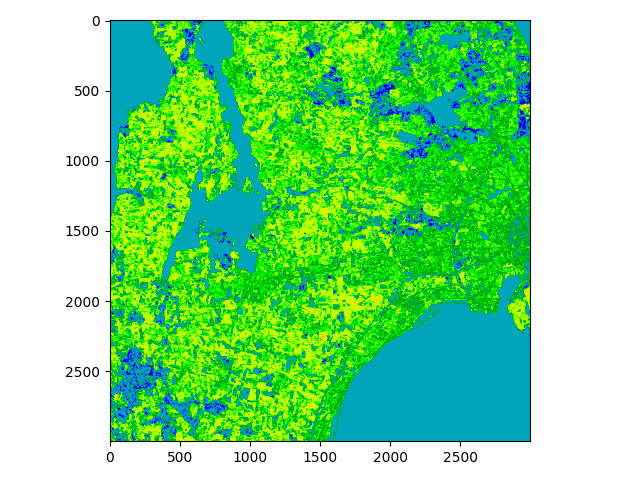
\includegraphics[width=\textwidth]{figures/landsat_area_predictions.png}
  \vspace{-0.8cm}
  \caption{\small \textit{Plot of predicted labels for the}
  \texttt{landsat\_area.csv} \textit{dataset.}}
  \label{fig:landsat_area}
\end{figure}

The plot shows a satellite image of a part of eastern Sjælland, including half
of Copenhagen, some of Amager, Roskilde, Furesø, etc.

\subsubsection{Maximum depth/height of binary decision trees}

The maximum depth/height of a binary decision tree built over $n$ training data points
is $n - 1$ (using one-based counting). This worst-case scenario occurs when at
each internal node of the tree, the decision boundary is chosen such that the
training data $S$ is split into $L_{d, \theta}$ and $R_{d, \theta}$ with:
\begin{alignat}{3}
  &|L_{d, \theta}| = 1 &&\, \text{ and }\,  |R_{d, \theta}| = |S| - 1\\[6pt]
  \text{or }\quad &|L_{d, \theta}| = |S| - 1 &&\, \text{ and }\,  |R_{d, \theta}| =
  1\, .\label{eq:norm}
\end{alignat}

As an example, consider a training set with $n = 100$ training points. At the
root node, the training set is split into two sub-trees of size 1 and 99,
respectively. The size 1 sub-tree is trivially pure and is no longer split. The
set of points in the other sub-tree is split into two new sets of size 1 and 98.
This repeats another 97 times until the 99'th split which produces two sub-trees
of size 1.

\subsection{Normalization}

\paragraph{Transformation invariance of KNN}~\smallskip

For the nearest neighbour classifier to be invariant under some transformation
$f$ of the input space, we must have that the nearest neighbour relation of points
is preserved under $f$. In other words, if we have $\text{dist}(\mbf x, \mbf y)
\leq \text{dist}(\mbf x, \mbf z)$ for some vectors $\mbf x, \mbf y, \mbf z \in
\mathbb R^n$ and a monotone distance function $\text{dist}$, then
$f$ must satisfy:

\begin{align*}
  \text{dist}(\mbf x, \mbf y) \, \leq \, \text{dist}(\mbf x, \mbf z)\quad
  \Leftrightarrow \quad
  \text{dist}(f(\mbf x), f(\mbf y)) \, \leq\, \text{dist}(f(\mbf x), f(\mbf z)).
\end{align*}

This relationship is preserved whenever $f$ is monotonic\footnote{For the case
of $n > 1$, define monotonicity as such: $f$ is monotonic if $\forall i\,:\ a_i < b_i \iff
f(\mbf a)_i < f(\mbf b)_i$.}. However, to
illustrate, let $\text{dist}$ be Euclidean distance, and $f$ be the
normalization function:

\begin{align*}
  \text{dist}(\mbf a, \mbf b) &= \sqrt{\sum_{i = 1}^n \left(a_i - b_i\right)^2}, \\[4pt]
  f(\mbf a)_i &= \frac{a_i - \mu}{\sigma},
\end{align*}

where $\mu$ and $\sigma$ are the mean and standard deviation of the input set,
respectively. Then we have:

\begin{align*}
  \text{dist}(f(\mbf a), f(\mbf b)) &= \sqrt{\sum_{i = 1}^n \left(\frac{a_i -
  \mu}{\sigma}- \frac{b_i - \mu}{\sigma}\right)^2}\\[4pt]
  &= \sqrt{\frac{1}{\sigma}\sum_{i = 1}^n \left(a_i - b_i\right)^2}\\[4pt]
\end{align*}

Since $\sigma$ is always non-negative, the square root is still defined.
Plugging this into \cref{eq:norm}:

\begin{alignat*}{3}
  &\sqrt{\sum_{i = 1}^n \left(a_i - b_i\right)^2} &&\quad \leq\quad  \sqrt{\sum_{i = 1}^n
  \left(a_i - b_i\right)^2}\\[4pt]
  \Leftrightarrow\quad  &\sqrt{\frac{1}{\sigma}\sum_{i = 1}^n \left(a_i -
  b_i\right)^2} &&\quad \leq\quad  \sqrt{\frac{1}{\sigma}\sum_{i = 1}^n \left(a_i - b_i\right)^2}
  \\[4pt]
\end{alignat*}

We see that the nearest-neighbour relation is preserved under $f$.


\paragraph{Transformation invariance of Random Forests}~\smallskip

Similar reasoning applies to the case of Random Forests. At each internal node
of each tree in the Random Forest, some comparison $a \leq b$ is made, and if
$f$ is a monotone function then $a \leq b$ again implies $f(a) \leq f(b)$.

\sectend
 % DONE

\newpage

\section{Logistic Regression}


\subsection{Cross-entropy error measure}

\subsubsection{Part (a)}

In the maximum likelihood method, we want to maximize the likelihood -- but
instead of differentiating a product, we instead maximize the log-likelihood
\textit{or}, as I will do, minimize its negative, which amounts to
differentiating the negative log-likelihood function given by:

\begin{align}
  - \sum_{n = 1}^N \lnb{\PP{y_n | x_n}}\label{eq:log_likelihood}
\end{align}

For logistic regression with labels $Y \in \{-1, 1\}$, we have: 

\begin{align*}
  \PP{Y = y\ |\ X = x} = 
\begin{cases}
  h(x),\quad &y = 1\\
  1 - h(x),\quad &y = -1
\end{cases}
\end{align*}

Using the indicator function, the above definition can be rewritten into
something which is not piecewise but which still splits the two cases
rewritten into something that allows us to split the two cases (note the use of
bracket notation for the indicator function, as in Abu Mostafa):

\begin{align*}
  \PP{Y = y\ |\ X = x}\ =\ \booltoint{y = 1} * h(x)\ +\ \booltoint{y = -1} * (1 -
  h(x))
\end{align*}

And then \cref{eq:log_likelihood} becomes:

\begin{align*}
  - \sum_{n = 1}^N \left(\booltoint{y_n = 1}\lnb{h(x)}\ +\ \booltoint{y_n = -1} \lnb{1 -
  h(x)}\right).
\end{align*}

Using $\lnb{a} = -\lnb{a^{-1}}$:
\begin{align}
  \sum_{n = 1}^N \left(\booltoint{y_n = 1} \lnb{\frac{1}{h(x)}}\ +\
  \booltoint{y_n =
  -1}\lnb{\frac{1}{1 - h(x)}}\right).
  \label{eq:end_part_a}
\end{align}
\qed

\subsubsection{Part (b)}

\noindent For the case $h(\mbf x) = \mysigx$, we have:
\begin{align*}
  \lnb{\frac{1}{\mysigx}}    &= \lnb{1 + e^{-\mbf w^{\text{T}} \mbf x_n}},\\[6pt]
  \lnb{\frac{1}{1 - \mysigx}} &= \lnb{1 + e^{\mbf w^{\text{T}} \mbf x_n}}.
\end{align*}

\noindent Substituting this into \cref{eq:end_part_a}, we get:

\begin{align*}
  \sum_{n = 1}^N \left(\booltoint{y_n = 1} \lnb{1 + e^{-\mbf w^{\text{T}} \mbf x_n}}\ +\ \booltoint{y_n =
  -1}\lnb{1 + e^{\mbf w^{\text{T}} \mbf x_n}}\right).
\end{align*}

\noindent At this point, please note that:
\begin{align*}
  \lnb{1 + e^{-\mbf w^{\text{T}} \mbf x_n}} = \lnb{1 + e^{-y_n \mbf w^{\text{T}} \mbf x_n}}, \quad
  &\text{when } y_n = 1,\\[4pt]
  \lnb{1 + e^{\mbf w^{\text{T}} \mbf x_n}} = \lnb{1 + e^{-y_n \mbf w^{\text{T}} \mbf x_n}}, \quad
  &\text{when } y_n = -1.
\end{align*}

\noindent Using this knowledge we can collapse the terms in the logairhtm as
such:

\begin{align*}
  \sum_{n = 1}^N \lnb{1 + e^{-y_n\mbf w^{\text{T}} \mbf x_n}}.
\end{align*}

\noindent Finally, minimizing this function is equivalent to minimizing the same
function scaled by $\tfrac{1}{N}$, thus concluding the proof.
\qed
 % DONE

\newpage 
\subsection{Logistic regression loss gradient}

\subsubsection{Part 1 -- using \{-1, 1\} labels}

The gradient I want to compute is:

\begin{align*}
  \nabla_{\mbf w} E_\text{in}(\mbf w) &= \ddw \meanN \lnb{1 + e^{-\ywx}}
\end{align*}

\noindent For labels $Y \in \{-1, 1\}$.

First I use the constant rule as well as the summation rule for differentiation
to move the derivative inside:

\begin{align*}
  &= \meanN \ddw \lnb{1 + e^{-\ywx}}
\end{align*}

\noindent Using $\tfrac{d}{dx}\ln (f(x)) = f(x)^{-1} * \tfrac{d}{dx} f(x)$:

\begin{align*}
  &= \meanN \frac{1}{1 + e^{-\ywx}} * \tddw\left(1 + e^{-\ywx}\right)\\
\end{align*}

\noindent And next, the exponent rule for differentiation:

\begin{align*}
  &= \meanN \frac{1}{1 + e^{-\ywx}} * (- y_n) \mbf x_n (1 + e^{-\ywx})\\
  &= \meanN \frac{1}{1 + e^{\ywx}} * (- y_n) \mbf x_n
\end{align*}

\noindent Finally, I use the definition of the Sigmoid function to conclude the
proof:

\begin{align*}
  &= \meanN - y_n \mbf x_n \theta\!\left[-y_n \mbf w^{\text{T}}\mbf x_n\right].
\end{align*}
\qed

When a label $y_n$ is mispredicted, we have $\ywx < 0$ and thus $-\ywx > 0$ and
$\theta\left[-\ywx\right] > 0.5$ -- conversely, when $y_n$ is correctly
classified, we have $\theta\left[-\ywx\right] < 0.5$, meaning misclassifications
contribute more than correct classifications.

\subsubsection{Part 2 -- using \{0, 1\} labels}

First I define the distribution $\P (Y = y \, |\, X = x)$ given labels $Y \in \{0,
1\}$ in terms of the sigmoid function:

\begin{align*}
  \P(Y = y\,|\,X = \mbf x) = 
  \begin{cases}
    \mysigx,     &y = 1\\
    1 - \mysigx, &y = 0
  \end{cases}
\end{align*}

With some clever use of the indicator function, I rewrite the above to something
that will be more useful in a moment:

\begin{align*}
  \P(Y = y\,|\,X = x) \ =\ \booltoint{y = 1} * \mysigx + \booltoint{y = 0} * \left(1 -
  \mysigx\right)
\end{align*}

However, since I know $Y$ to only take values 0 and 1, I can further substitute
exponentiation with 0 and 1 for the indicator function:

\begin{align*}
  \P(Y = y\,|\,X = x) \ =\ \mysigx^y * \left(1 - \mysigx\right)^{1 - y}
\end{align*}

This rewrite is going to be useful in a moment, once I start manipulating logarithms.

Using $\P $ as defined above, the problem I want to solve is the derivative wrt.
$\mbf w$ of below log-likelihood:

\begin{align*}
  \nabla_{\mbf w} E_\text{in}(\mbf w)&= \ddw \meanN\Big( \lnb{\mysig^{y_n} *
  \left(1 - \mysig\right)^{1 - y_n}}\Big)
  % \nabla_{\mbf w} E_\text{in}(\mbf w)&= \ddw \meanN\Big( \lnb{\mysig^{y_n}} +
  % \lnb{\left(1 - \mysig\right)^{1 - y_n}}\Big)
\end{align*}

\noindent Using first $\ln (ab) = \ln (a) + \ln (b)$ and $\ln (x^y) = y \ln (x)$:
\begin{align*}
  &= \ddw \meanN\Big( y_n * \lnb{\mysig} +
  (1 - y_n) * \lnb{1 - \mysig}\Big)
\end{align*}

\noindent Using the constant rule and summation rule for differentiation:

\begin{align*}
  &= \meanN\ddw \Big(y_n \lnb{\mysig} + (1 - y_n)\lnb{1 - \mysig}\Big)\\[4pt]
  &= \meanN \Big(y_n \tddw \lnb{\mysig} + (1 - y_n) \, \tddw \lnb{1 - \mysig}\Big)
\end{align*}

\noindent Using $\tfrac{d}{dx} \lnb{f(x)} = \tfrac{1}{f(x)} * \tfrac{d}{dx} f(x)$:

\begin{align*}
  &= \meanN \Big(
  y_n * \frac{1}{\mysig} * \tddw \mysig + (1 - y_n) * \frac{1}{1 - \mysig} * \tddw
  \left(1 - \mysig\right)
  \Big)
\end{align*}

Moving factors onto numerators and outside of the last differential; then
factoring:

\begin{align*}
  &= \meanN \Big(
  \frac{y_n}{\mysig} * \tddw \mysig - \frac{1 - y_n}{1 - \mysig} * \tddw
  \mysig
  \Big)\\[4pt]
  &= \meanN \Big(
  \frac{y_n}{\mysig} - \frac{1 - y_n}{1 - \mysig}
  \Big) * \tddw \mysig
\end{align*}

At this point I use the fact that $\tfrac{d}{dx}\theta\!\left[x\right] =
\theta\!\left[x\right] * (1 - \theta\!\left[x\right])$ in conjunction with the
exponent rule to compute $\tddw \mysig$:

\begin{align*}
  &= \meanN \Big(
  \frac{y_n}{\mysig} - \frac{1 - y_n}{1 - \mysig}
  \Big) * \mysig * (1 - \mysig) * \mbf x_n
\end{align*}

\noindent Using some basic algebra to compute the difference of fractions:

\begin{align*}
  &= \meanN \Big(
  \frac{y_n - \mysig}{\mysig * (1 - \mysig)}
  \Big) * \mysig * (1 - \mysig) * \mbf x_n
\end{align*}

\noindent The denominator cancels out to conclude the proof:

\begin{align*}
  \meanN \left(
  y_n - \mysig
  \right) * \mbf x_n\ = \ \nabla_{\mbf w} E_\text{in}(\mbf w)
\end{align*}
\qed


\newcommand{\wz}{\mbf w_0}
\newcommand{\wo}{\mbf w_1}
\newcommand{\wzt}{\mbf w_0^{\text{T}}}
\newcommand{\wot}{\mbf w_1^{\text{T}}}
\newcommand{\wztx}{\mbf w_0^{\text{T}} \mbf x_n}
\newcommand{\wotx}{\mbf w_1^{\text{T}} \mbf x_n}
\newcommand{\norm}[1]{\left\lVert#1\right\rVert}
\newcommand{\abs}[1]{\left|#1\right|}


To see how misclassifications contribute more to the gradient of
$E_{\text{in}}(\mbf w)$, let $\wz$ and $\wo$ be two vectors which, when
dotted with $\mbf x_n$, correspond to classifications of 0 and 1, respectively.
In other words, let $\wz$ and $\wo$ be vectors such that:

\begin{align*}
  \wzt \mbf x_n &< 0\\
  \wot \mbf x_n &\geq 0
\end{align*}

and thus:

\begin{align}
  0\ \leq\ \theta[\wztx]\ <\ 0.5\ \leq\ \theta[\wotx]\ \leq\ 1.\label{eq:thetas}
\end{align}

Now, assume $y_n = 1$, and let's examine the relationship between the
contribution to the gradient of guessing 0 vs. guessing 1:

\begin{alignat*}{2}
  \norm{\underbrace{\big(1 - \theta[\wzt \mbf x_n]\big)\ \mbf x_n
  }_{\text{guessing 0 for } y_n =\; 1}}\ &\mygeq\ \norm{\underbrace{\big(1 - \theta[\wot \mbf
  x_n]\big)\ \mbf x_n}_{\text{guessing 1 for } y_n =\; 1}}\\[4pt]
\end{alignat*}

Using first $\lVert a * \mbf y\rVert = |a| * \lVert \mbf y \rVert$:

\begin{alignat*}{2}
  \Leftrightarrow\quad\abs{1 - \theta[\wzt \mbf x_n]} * \norm{\mbf x_n
  }\quad &\mygeq\quad \abs{1 - \theta[\wot \mbf x_n]} *\norm{\mbf x_n}\\[4pt]
  \Leftrightarrow\quad\abs{1 - \theta[\wzt \mbf x_n]} \quad &\mygeq\quad \abs{1 - \theta[\wot \mbf x_n]}
\end{alignat*}

Since $\theta[s] \in [0, 1]$ for any $s$, we know that the values
in these absolute operators are always non-negative, so we can safely remove the
absolute value operators:

\begin{align*}
  \Leftrightarrow\quad1 - \theta[\wzt \mbf x_n] \quad &\mygeq\quad
  1 - \theta[\wot \mbf x_n]\\[4pt]
  \Leftrightarrow\quad- \theta[\wzt \mbf x_n] \quad &\mygeq\quad
  - \theta[\wot \mbf x_n]\\[4pt]
  \Leftrightarrow\quad \theta[\wzt \mbf x_n] \quad &\leq\quad
  \theta[\wot \mbf x_n]
\end{align*}

The arrived at equality is true as per \cref{eq:thetas}, and thus we see that if
$y_n = 1$, then guessing 0 yields a larger contribution to the gradient than
does guessing 1.

% \smallskip\noindent\makebox[\textwidth]{\rule{\textwidth}{0.3pt}}

\bigskip

\bigskip

\noindent Conversely, assume now $y_n = 0$. Then we have the following inequality:
\begin{alignat*}{2}
  \norm{\underbrace{\big(0 - \theta[\wzt \mbf x_n]\big)\ \mbf x_n
  }_{\text{guessing 0 for } y_n =\; 0}}\ &\myleq\ \norm{\underbrace{\big(0 - \theta[\wot \mbf
  x_n]\big)\ \mbf x_n}_{\text{guessing 1 for }y_n =\; 0}  }\\[6pt]
  \Leftrightarrow\quad
   \norm{- \mbf x_n \theta[\wzt \mbf x_n] }\  &\myleq\ \norm{- \mbf x_n \theta[\wot \mbf x_n] }
\end{alignat*}

\smallskip

Using $\lVert \mbf y * b\rVert = \lVert \mbf y \rVert * |b|$:
\begin{align*}
  \Leftrightarrow\quad\norm{- \mbf x_n }\abs{\theta[\wzt \mbf x_n]} \  &\myleq\
  \norm{- \mbf x_n  }\abs{\theta[\wot \mbf x_n]}\\[4pt]
   \Leftrightarrow\quad\abs{\theta[\wzt \mbf x_n]} \  &\myleq\ \abs{\theta[\wot \mbf
   x_n]}\\[4pt]
\end{align*}

Using again non-negativity of the sigmoid function to remove absolute operators,
and \cref{eq:thetas} to verify the inequality:

\begin{align*}
   \Leftrightarrow\quad\theta[\wzt \mbf x_n] \  &\leq\ \theta[\wot \mbf
   x_n]
\end{align*}

Once again we arrive back at the assumption, so here we see that if $y_n = 0$,
then guessing 1 contributes more to the gradient than guessing 1.

\qed

\sectend
 % DONE
\newpage
\newcommand{\ea}{e^{\mbf w ^{\text{T}} \mbf x + b}}
\newcommand{\eam}{e^{-(\mbf w ^{\text{T}} \mbf x + b)}}


\subsection{Log-odds}

Starting from the definition of $\mbf w ^{\text{T}} + b$ assuming log-odd
encoding (as given in equation (2) in the assignment text), I use $e^{\lnb{a}} =
a$ and some basic arithmetic to manipulate the expression:


\begin{align*}
  \mbf w ^{\text{T}} \mbf x+ b\ &=\ \lnb{\frac{\PP{Y = 1\ |\ X = x}}{\PP{Y = 0\ |\ X =
  x}}}\\[4pt]
  e^{\mbf w ^{\text{T}}\mbf x + b}\ &=\ \frac{\PP{Y = 1\ |\ X = x}}{\PP{Y = 0\ |\ X =
  x}}\\[4pt]
  \PP{Y = 0\ |\ X = x}\ e^{\mbf w ^{\text{T}}\mbf x + b}\ &=\ \PP{Y = 1\ |\ X =
  x}\\[4pt]
   (1 - \PP{Y = 1\ |\ X = x})\ e^{\mbf w ^{\text{T}}\mbf x + b}\ &=\ \PP{Y = 1\
   |\ X = x}
\end{align*}

\noindent Using $\sigma(\mbf w ^{\text{T}} \mbf x + b) = \PP{Y = 1\ |\ X = x}$ as per
equation (1) in the assignment text:

\begin{align*}
   (1 - \sigma(\mbf w ^{\text{T}} \mbf x + b))\ e^{\mbf w ^{\text{T}}\mbf x + b}\ &=\ \sigma(\mbf w ^{\text{T}} \mbf x + b)
\end{align*}

If $\sigma$ is, in fact, the logistic (sigmoid) function, then the above
equation should hold once we substitute in its definition:

\begin{align*}
  \left(1 - \frac{1}{1 + \eam}\right)\ e^{\mbf w
   ^{\text{T}}\mbf x + b}\ &\myeq\ \frac{1}{1 + \eam}\\
\end{align*}

Using distributivity of multiplication:

\begin{align*}
\Leftrightarrow\quad \ea - \frac{\ea}{1 + \eam} &\myeq \ \frac{1}{1 + \eam}\\[4pt]
\end{align*}

Now, using the magic algebraic rule $\frac{a}{b + c} = \frac{a}{b} -
\frac{ac}{b(b + c)}$ to split the fraction on the LHS of the equation in two:

\begin{align*}
  \Leftrightarrow\quad \ea - (\ea - \frac{\ea * \eam}{1 + \eam})&\myeq \ \frac{1}{1 + \eam}\\[4pt]
  \Leftrightarrow\quad \ea - (\ea - \frac{1}{1 + \eam})&\myeq \ \frac{1}{1 + \eam}\\[4pt]
  \Leftrightarrow\quad \ea - \ea + \frac{1}{1 + \eam}&\myeq \ \frac{1}{1 + \eam}\\[4pt]
  \Leftrightarrow\quad \frac{1}{1 + \eam} &= \ \frac{1}{1 + \eam}
\end{align*}

I find that the equality holds, and thus I conclude the proof.

\qed

\sectend
 % DONE

\end{document}
